いま鋭角の仮説をとる。平面上で第三の直線に垂直な二直線は、その共通の垂線の両側で互いに離れてゆく。三角形の角の和は二直角より小さく、前章の命題は制限なしに成り立つ。

\section{平行線}

任意の点 $P$ から、与えられた直線 $AB$ へ垂線 $PC$ を引き、$P$ から $CB$ 上の点 $D$ へ別の線 $PD$ を引く。$D$ が $CB$ 上を限りなく遠ざかってゆくと、線 $PD$ はある極限の位置 $PE$ に近づく。

\begin{figure}[h]
\centering
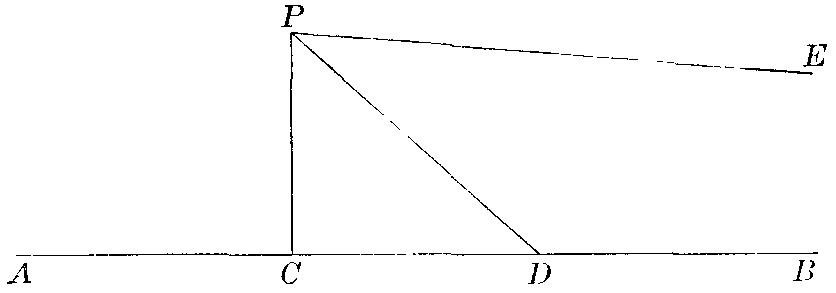
\includegraphics[width=80mm]{fig28.png}
\end{figure}

$PE$ は、$P$ において $CB$ に\emph{平行}であるという。$PE$ が $PC$ となす角 $CPE$ を、垂直距離 $PC$ に対する\emph{平行角}という。それは直角より小さく、小さい量は三角形 $PCD$ の不足の極限である。$PC$ の反対側にも、$CA$ に平行で、$PC$ と同じ平行角をなす別の線を見いだすことができる。$PE$ は、$PC$ に関して $PE$ と同じ側にある部分に向かって $AB$ に平行であるという。このように、任意の点において、一つの直線に対する平行線は二本あるが、直線の一方の向きに対しては一本だけである。$P$ を通る線で、$PC$ とのなす角が平行角より大きく、かつその補角より小さいものは、$AB$ とまったく交わらない。垂直距離 $p$ に対する平行角を $\Pi(p)$ と書く。

\begin{description}
\item[1.~定理.] \emph{直線は、すべての点においてその平行性を保つ。}

\begin{figure}[h]
\centering
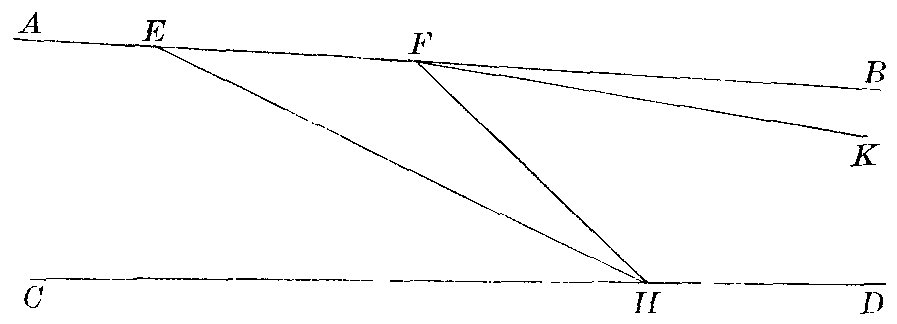
\includegraphics[width=80mm]{fig29.png}
\end{figure}

\textbf{$AB$} が $E$ において $CD$ に平行であるとし、$E$ の両側の $AB$ 上の任意の他の点を $F$ とするとき、$AB$ が $F$ においても $CD$ に平行であることを証明する。

\textbf{証明.} $CD$ 上の $H$ に、$EH$ と $FH$ を引く。$H$ が $CD$ 上を限りなく遠ざかると、これら二つの線は $CD$ に平行な位置に近づく。しかし $EH$ の極限の位置は、$F$ を通る直線 $AB$ であり、もし $FH$ の極限の位置が別の線 $FK$ であるとすれば、$F$ が、$EH$ と $FH$ の交点である $H$ の極限の位置になってしまう。

\item[2.~定理.] \emph{一つの直線が他の直線に平行ならば、第二の直線は第一の直線に平行である。}

\textbf{$AB$} が $CD$ に平行であるとき、$CD$ が $AB$ に平行であることを証明する。

\textbf{証明.} $CD$ に垂直に $AC$ を引く。角 $CAB$ は鋭角である。したがって、$C$ から $AB$ へ下ろした垂線 $CE$ は、直線 $AB$ が $CD$ に平行である向きの側の、$A$ の側に落ちなければならない（第I章, II, 1）。そのとき角 $ECD$ は鋭角で、直角である $CEB$ より小さい。すなわち、
\begin{equation*}
CAB < ACD, \quad \text{かつ} \quad CEB > ECD
\end{equation*}
である。

線 $CE$ が点 $C$ のまわりに $CA$ の位置まで回転すると、$E$ での角は角 $A$ まで減少し、$C$ での角は直角まで増加する。この二つの角が等しくなる位置が、たとえば $CF$ にある。すなわち、
\begin{equation*}
CFB = FCD
\end{equation*}
である。

\begin{figure}[h]
\centering
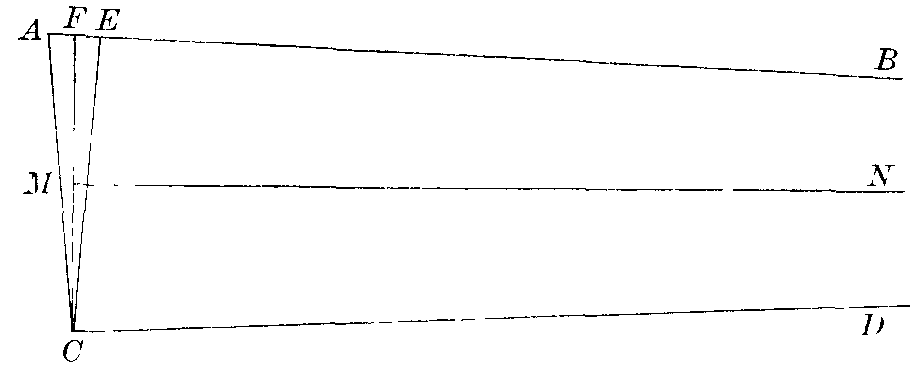
\includegraphics[width=80mm]{fig30.png}
\end{figure}

$CF$ の中点で $CF$ に垂直に $MN$ を引き、図形を $MN$ を軸として回転させる。$CD$ は $AB$ のもとの位置に重なり、$AB$ は $CD$ のもとの位置に重なる。したがって、$CD$ は $AB$ に平行である。

\textbf{系.} \emph{$FB$ と $CD$ は、ともに $MN$ に平行である。}

\begin{figure}[h]
\centering
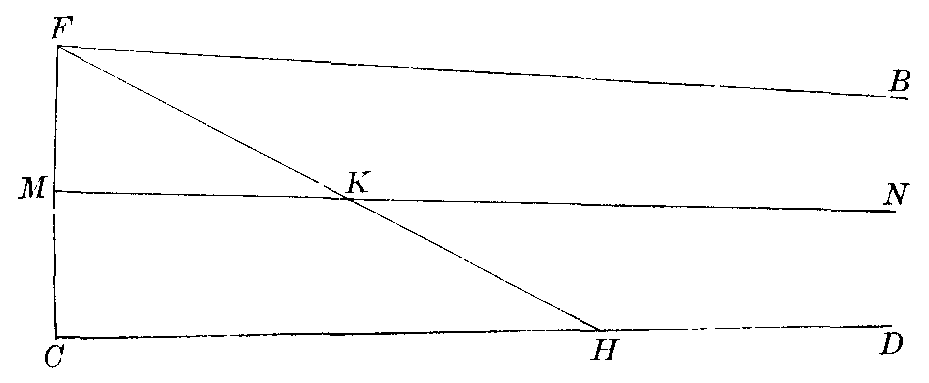
\includegraphics[width=80mm]{fig31.png}
\end{figure}

\textbf{証明.} $FB$ と $CD$ は $MN$ に関して対称の位置にあり、互いに交わらないから、$MN$ とも交わらない。$CD$ 上の $H$ に $FH$ を引き、$MN$ と $K$ で交わるとする。$H$ が $CD$ 上を限りなく遠ざかると、$FH$ は極限として $FB$ の位置に近づく。ところで、$K$ が $H$ より先に限りなく遠ざかることはできない。$FK < FH$ だからである。しかしまた、$H$ が限りなく遠ざかるとき、$K$ が $MN$ 上の有限の距離にある極限の位置に近づくこともできない。そうなれば、$FB$、したがって $CD$ は、この点で $MN$ と交わり、互いにも交わることになるからである。ゆえに $H$ と $K$ は一緒に遠ざからなければならず、$FH$ の極限の位置は、同時に $CD$ と $MN$ に平行でなければならない。

同様にして、平面上で二本の平行線の間にある任意の線は、そのどちらかと交わるか、両方に平行であることを証明できる。

\item[3.~定理.] \emph{第三の直線の同じ向きに対してそれに平行な二直線は、互いに平行である。}

\begin{figure}[h]
\centering
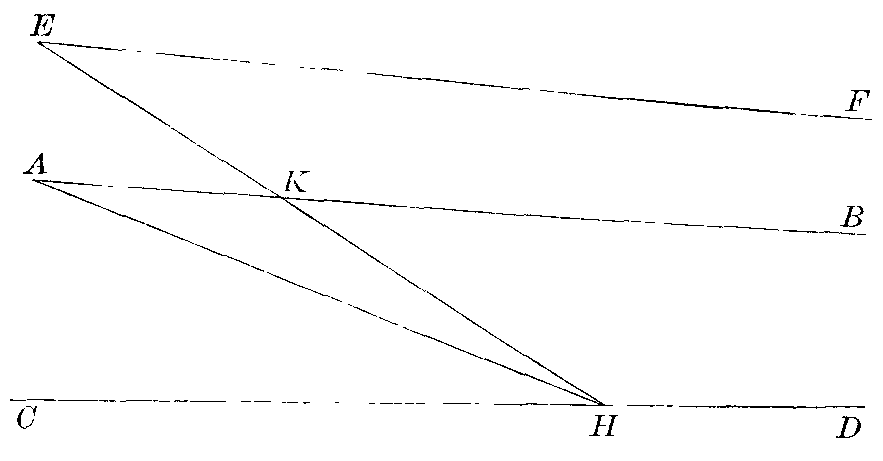
\includegraphics[width=80mm]{fig32.png}
\end{figure}

\textbf{第一に、}すべてが同じ平面にあるとき。

\textbf{$AB$} と $EF$ が $CD$ に平行であるとき、それらが互いに平行であることを証明する。

\textbf{証明.} $AB$ が他の二直線の間にあるとする。$CD$ 上の任意の点 $H$ に $AH$ と $EH$ を引き、$EH$ が $AB$ と交わる点を $K$ とする。$H$ が $CD$ 上を限りなく遠ざかるとき、$AH$ と $EH$ は極限の位置として $AB$ と $EF$ に近づく。ところで、$K$ が $H$ より先に限りなく遠ざかることはできない。$EK < EH$ だからである。しかしまた、$H$ が限りなく遠ざかるとき、$K$ が $AB$ 上の有限の距離にある極限の位置に近づくこともできない。この点は $AB$ と $EF$ の交点であり、$H$ の極限の位置でもあることになるが、$H$ は $CD$ 上を限りなく遠ざかるからである。ゆえに $H$ と $K$ は一緒に遠ざからなければならず、$EH$ の極限の位置は同時に $CD$ と $AB$ に平行でなければならない。

他の二直線の間にある $AB$ が、$CD$ と $EF$ に平行であると与えられているならば、$EF$ は $CD$ に平行でなければならない。$E$ を通って $CD$ に平行な線は $AB$ に平行であり、同じ向きに対して $E$ を通って $AB$ に平行な線は一本しか引けないからである。

\begin{figure}[h]
\centering
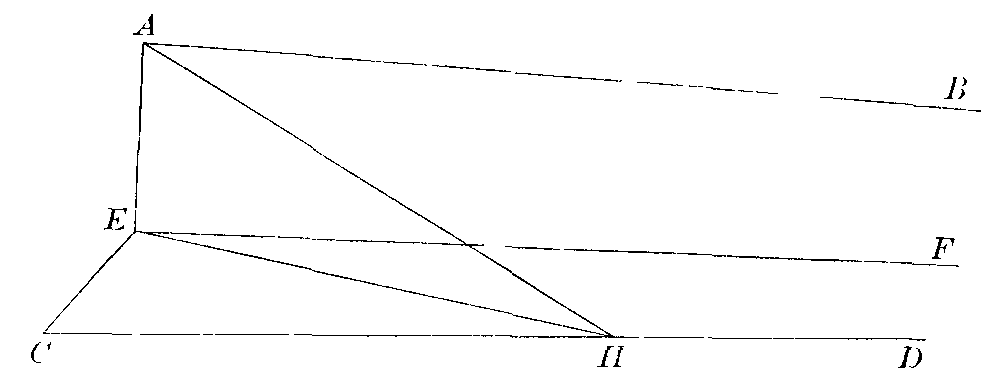
\includegraphics[width=80mm]{fig33.png}
\end{figure}

\textbf{第二に、}直線がすべて同じ平面にないとき。

\textbf{$AB$} と $CD$ を二本の平行線とし、$E$ をそれらの平面にない任意の点とする。

\textbf{証明.} $CD$ 上の $H$ に、$AH$ と $EH$ を引く。$H$ が限りなく遠ざかるとき、$AH$ は $AB$ の位置に近づき、平面 $EAH$ は平面 $EAB$ の位置に近づく。したがって、$EH$ の極限の位置は平面 $ECD$ と $EAB$ の交線である。そうするとこれらの平面の交線は $CD$ に平行であり、同様にして、それが $AB$ にも平行であることが証明される。

さて、$EF$ がこの二直線の一方に、それらが平行である向きに対して平行であると与えられているならば、それは、それらと点 $E$ とによって定まる二つの平面の交線でなければならず、したがって他方の直線にも平行である。

\item[4.~定理.] \emph{平行線は互いに近づきつづける。}

\textbf{$AB$} と $CD$ が平行であるとし、$AB$ 上の任意の点 $A$ と $B$ から、$CD$ へ垂線 $AC$ と $BD$ を下ろす。$B$ が平行の向きに関して $A$ の先にあるとして、$BD < AC$ を証明する。

\textbf{証明.} $CD$ の中点 $H$ に、$AB$ と $K$ で交わる垂線を立てる。角 $BKH$ は鋭角であり、角 $AKH$ は鈍角である。したがって、$K$ で $HK$ に垂直な線は、$CA$ と $C$ と $A$ の間のある点 $E$ で、延長した $DB$ と $B$ の先のある点 $F$ で交わらなければならない。しかるに $DF = CE$（第I章, I, 12）であるから、$DB < CA$ である。

\begin{figure}[h]
\centering
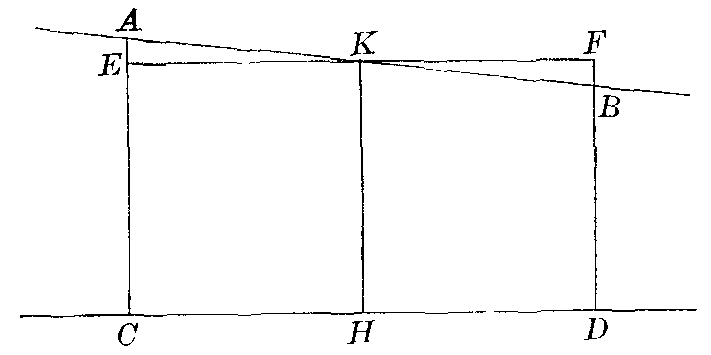
\includegraphics[width=80mm]{fig34.png}
\end{figure}

\textbf{系.} \emph{$AB$ と $CD$ が平行で、$AC$ がそれらと等しい角をなす（上の 2 の $FC$ のような）ならば、この二直線上に等しい距離 $AE = CF$ を、それらが平行である向きの側に切り取る $EF$ は、$AC$ より短い。}

\begin{figure}[h]
\centering
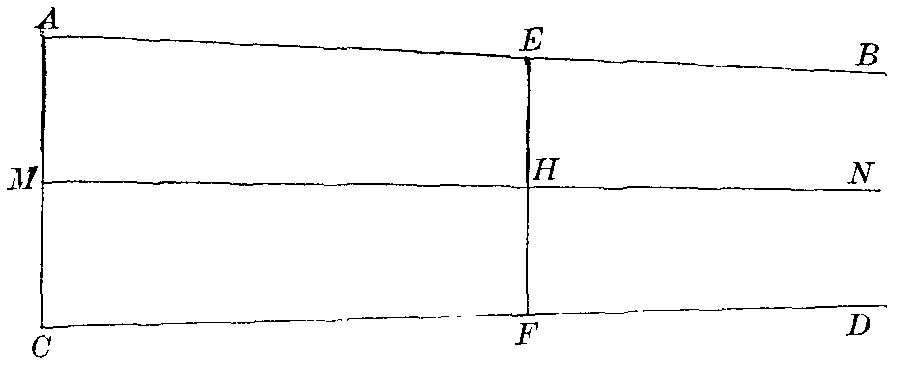
\includegraphics[width=80mm]{fig35.png}
\end{figure}

\textbf{証明.} $AC$ の中点で $AC$ に垂直な $MN$ は、$AB$ に平行で、$EF$ を二等分する。図形は $MN$ に関して対称だからである。$EF$ の半分である $EH$ は $AM$ より小さく、したがって $EF$ は $AC$ より小さい。

\item[5.~定理.] \emph{垂直距離が零から出発して限りなく増加するとき、平行角は直角から零まで減少する。}

\textbf{証明.} まず第一に、平行角は、垂直距離が正である間は鋭角であるが、垂直距離を十分に小さくとれば、直角との差をどんな指定された値よりも小さくできる。

\begin{figure}[ht]
\centering
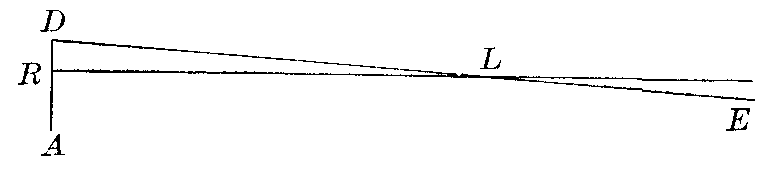
\includegraphics[width=70mm]{fig36.png}
\end{figure}

実際、$ADE$ を、望むだけ直角に近い任意の角とするとき、$DE$ 上に点 $L$ をとり、$LR$ を $R$ で $DA$ に垂直に引くことができる。角 $RDL$ は、増加して、垂直距離 $RD$ に対する平行角となる。

\begin{figure}[h]
\centering
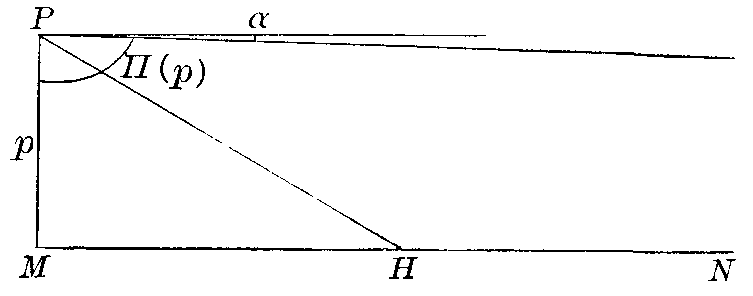
\includegraphics[width=70mm]{fig37.png}
\end{figure}

つぎに、$p$ を与えられた垂線 $PM$ の長さとし、$\alpha$ を、その平行角が $\frac{\pi}{2}$ と異なる量とする。すなわち、
\begin{equation*}
\Pi(p) = \frac{\pi}{2} - \alpha
\end{equation*}
とおく。$PM$ が $MN$ に垂直で、$H$ が $MN$ 上の任意の点であるとき、$H$ が $MN$ 上を限りなく遠ざかると、角 $MPH$ は極限として平行角 $\Pi(p)$ に近づく。線 $PH$ は、$MPH < \Pi(p)$ の間は線 $MN$ と交わり、$MPH$ を $\Pi(p)$ に十分近く、しかしそれより小さくとることによって、角 $MHP$ を望むだけ小さくできる（前章の該当ページを見よ）。

次ページの図（図38）において、$AC$ を $AB$ に垂直とし、$D$ を $AC$ 上の任意の点、$DE$ を $AB$ に平行な線とする。$DE$ の先に $DK$ を引き、$DE$ と角 $EDK=\Pi(p)$ をなすようにし、$DK = p$ とする。$K$ で $DK$ に垂直な $TF$ は、$DE$ と $AB$ に平行になる。

前の図の $PM$ を $DKT$ の上に置くことにより、
\begin{gather*}
KDC < \Pi(p), \\
\intertext{すなわち}
ADE > 2\alpha
\end{gather*}
ならば、$DC$ は $KT$ と点 $G$ で交わることがわかる。

そのとき直角三角形 $DKG$ において、
\begin{gather*}
DGK + KDG < \frac{\pi}{2}. \\
\intertext{しかるに}
ADE + KDG = \frac{\pi}{2} + \alpha; \\
\intertext{したがって、}
DGK < ADG - \alpha.
\end{gather*}

\begin{figure}[h]
\centering
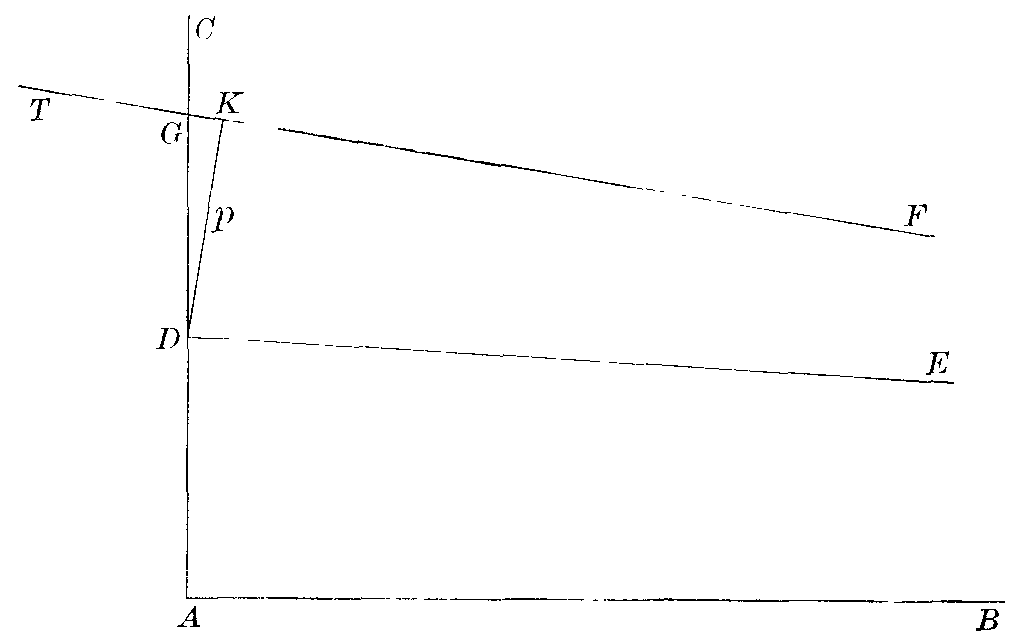
\includegraphics[width=80mm]{fig38.png}
\end{figure}

点 $G$ から出発して、この作図をくり返すことができ、そのたびに平行角から $\alpha$ より大きい量を引く。この過程は、平行角が $2\alpha$ に等しいか、それより小さくなるまで続けることができる。

点 $D$ が $AC$ に沿って動き、$DE$ が $AB$ に平行であるままならば、$D$ での角は絶えず減少し、$D$ を $AC$ に沿って十分遠くまで動かすことによって、この角が $2\alpha$ に等しいか、それより小さくなる点に達することができる。

$D$ が、平行角がちょうど $2\alpha$ となる点にあるとする。そこで、前と同様に $DK$ と $TF$ を引くと、$KT$ は $DC$ に平行になる。$AB$ とこの位置の $TF$ との間にある $AB$ へのすべての平行線は $AC$ と交わり、平行線がこの位置の $TF$ に近づくにつれて、$D$ での平行角は零に近づき、点 $D$ は限りなく遠ざかる。

\begin{figure}[h]
\centering
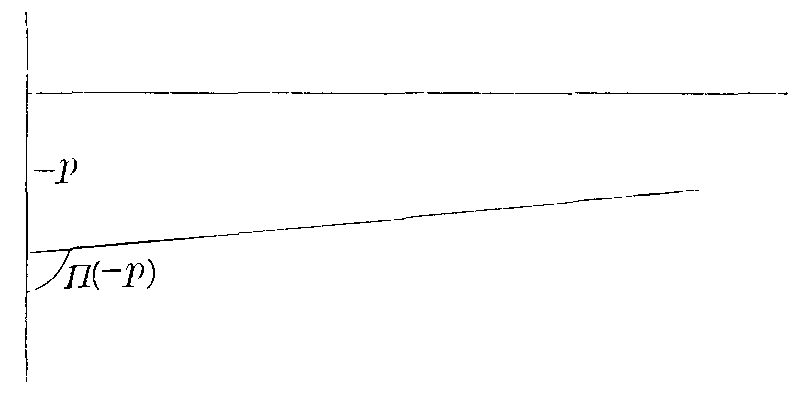
\includegraphics[width=60mm]{fig39.png}
\end{figure}

鈍角については、$p$ を負にとることができて、
\begin{equation*}
\Pi(-p) = \pi - \Pi(p)
\end{equation*}
である。

